% =============================================
% =============================================
% Document class: Beamer
\documentclass[ 10pt, xcolor = dvipsnames]{beamer}
% Packages: Beamer
\usepackage{ beamerthemesplit, lmodern}
\setbeamertemplate{frametitle continuation}{}
% Packages: LaTeX (Depth-1)
\usepackage[ linesnumbered, ruled, vlined]{algorithm2e}
\usepackage{ amsfonts, amsmath, amssymb, amsthm}
\usepackage{ color, colortbl}
\usepackage{ dsfont}
\usepackage{ float}
\usepackage{ hhline}
\usepackage{ graphicx}
\usepackage{ latexsym}
\usepackage{ mathtools, multicol, multirow}
\usepackage{ parskip, pbox, pifont}
\usepackage{ ragged2e}
\usepackage{ setspace, stmaryrd, subcaption}
\usepackage{ tabularx}
\usepackage{ wasysym}
% Packages: LaTeX (Depth-2)
\usepackage{ epstopdf}

% =============================================
% Themes, colors and styles
\hypersetup{ colorlinks, linkcolor =, urlcolor = blue, citecolor = blue}
\usetheme{Madrid}
\usecolortheme[named=Brown]{structure}
\useinnertheme{rectangles}
\beamertemplatenavigationsymbolsempty

% =============================================
% =============================================
% Macros: Language
\newcommand{\define}{\triangleq}
\newcommand{\done}{\hfill $\square$}
%\newcommand{\eqCIRC}{\stackrel{\circ}{=}}
%\newcommand{\eqSTAR}{\stackrel{*}{=}}
\renewcommand{\epsilon}{\varepsilon}
\newcommand{\eg}{\textit{e.g.,\;}}
\newcommand{\egc}{\textit{e.g.:\;}}
\newcommand{\Eg}{\textit{E.g.,\;}}
\newcommand{\Egc}{\textit{E.g.:\;}}
\newcommand{\ie}{\textit{i.e.,\;}}
\newcommand{\iec}{\textit{i.e.:\;}}
\newcommand{\Ie}{\textit{I.e.,\;}}
\newcommand{\Iec}{\textit{I.e.:\;}}
\newcommand{\QED}{\hfill $\blacksquare$}
\renewcommand{\tilde}[1]{\widetilde{#1}}
\newcommand{\tsup}[1]{\ensuremath{^{\text{#1}}}}
\newcommand{\tsub}[1]{\ensuremath{_{\text{#1}}}}
\renewcommand{\vec}[1]{{\boldsymbol{#1}}}

% Macros: Optimization & Probability
\DeclareMathOperator*{\argmax}{arg\,max}
\DeclareMathOperator*{\argmin}{arg\,min}
\newcommand{\Exp}{\mathbb{E}}
\newcommand{\Indicate}[1]{ \IndFun \, \{ \, #1 \, \} }
\renewcommand{\Pr}{\mathbb{P}}
\newcommand{\Normal}{\mathcal{N}}
\newcommand{\std}{\text{std}}
\newcommand{\var}{\text{var}}

% Macros: Sets
\newcommand{\Complex}{\mathbb{C}}
\renewcommand{\emptyset}{\varnothing}
\newcommand{\Nat}{\mathbb{N}}
\renewcommand{\Re}{\mathbb{R}}
\newcommand{\ReNN}{{\Re}_{\geq 0}}
\newcommand{\ReSP}{{\Re}_{> 0}}
\renewcommand{\subset}{\subseteq}
\renewcommand{\supset}{\supseteq}
\newcommand{\Z}{\mathbb{Z}}
\newcommand{\ZNN}{{\Z}_{\geq 0}}

% Macros: Spacing & Other Commands
\newcommand{\fullcut}{\vspace{-\baselineskip}}
\newcommand{\fullskip}{\vspace{\baselineskip}}
\newcommand{\halfcut}{\vspace{-0.5\baselineskip}}
\newcommand{\halfskip}{\vspace{0.5\baselineskip}}
\renewcommand{\figurename}{Figura}
\renewcommand{\tablename}{Tabla}

% =============================================
% =============================================
\title[Sistemas de Control: Unidad 01]{Sistemas de Control (EYAG-1005): \textbf{Unidad 01} }
\author[L. I. Reyes Castro]{Luis I. Reyes Castro}
\institute[ESPOL]{\normalsize Escuela Superior Polit\'ecnica del Litoral (ESPOL) \\ Guayaquil - Ecuador}
\date[2017-T1]{2017 - Primer T\'ermino}

\AtBeginSection[]
{
\begin{frame}
\frametitle{Contenido del Tema}
\tableofcontents[ currentsection, sectionstyle = show/shaded, subsectionstyle = show/show/hide]
\end{frame}
}
\AtBeginSubsection[]
{
\begin{frame}
\frametitle{Contenido del Tema}
\tableofcontents[ currentsection, currentsubsection, sectionstyle = show/shaded, subsectionstyle = show/shaded/hide]
\end{frame}
}

% =============================================
\begin{document}

% =============================================
\begin{frame}[noframenumbering]
\titlepage
\end{frame}
\begin{frame}[noframenumbering]
\frametitle{Contenido del Tema}
\tableofcontents[ subsectionstyle = hide]
\end{frame}

% =============================================
\section{Asuntos Administrativos}

% =============================================
\section{Conceptos B\'asicos}

% =============================================
\begin{frame}[allowframebreaks]
\frametitle{\insertsection: 1.3: System Configurations}

\begin{itemize}
\item Open Loop System: 
\begin{figure}
\centering
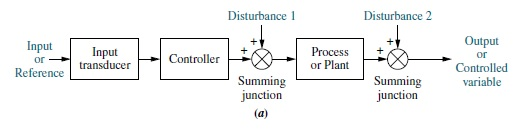
\includegraphics[ width = 0.7\textwidth]{fig_1-6a_open_loop_control.jpg}
\end{figure}
\item Closed Loop System: 
\begin{figure}
\centering
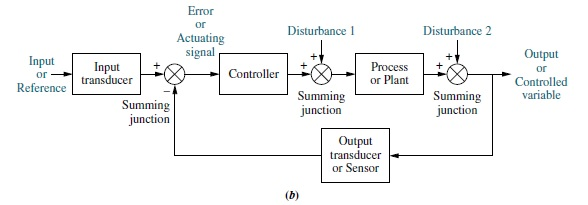
\includegraphics[ width = 0.7\textwidth]{fig_1-6b_closed_loop_control.jpg}
\end{figure}
\end{itemize}

\end{frame}

\end{document}

% =============================================
\begin{frame}[allowframebreaks]
\frametitle{\S 1.4: Analysis and Design Objectives}

\begin{itemize}
\item Analysis: 
\begin{itemize}
\item Process by which a system's performance is determined. 
\end{itemize}
\item Design: 
\begin{itemize}
\item Process by which a system's performance is created or changed. 
\end{itemize}
\item Major Objectives for Analysis and Design: 
\begin{itemize}
\item Stability
\item Transient Response
\item Steady-state Response
\item Other, \eg robustness to uncertainty in model parameters. 
\end{itemize}
\end{itemize}

\end{frame}

%% =============================================
%\begin{frame}[allowframebreaks]
%\frametitle{Control System Design Process}
%
%\begin{figure}
%\centering
%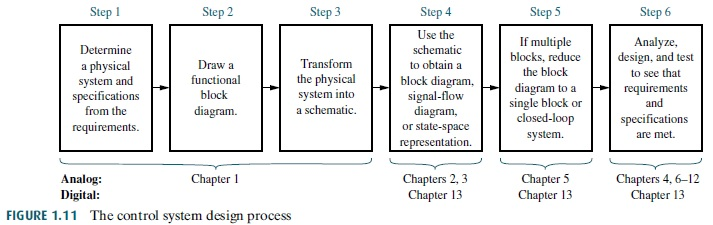
\includegraphics[ width = 0.98\textwidth]{fig_1-1-1_design_process.jpg}
%\end{figure}
%
%\end{frame}

% =============================================
\begin{frame}[allowframebreaks]
\frametitle{\S 1.5: Test Waveforms}

\begin{figure}
\centering
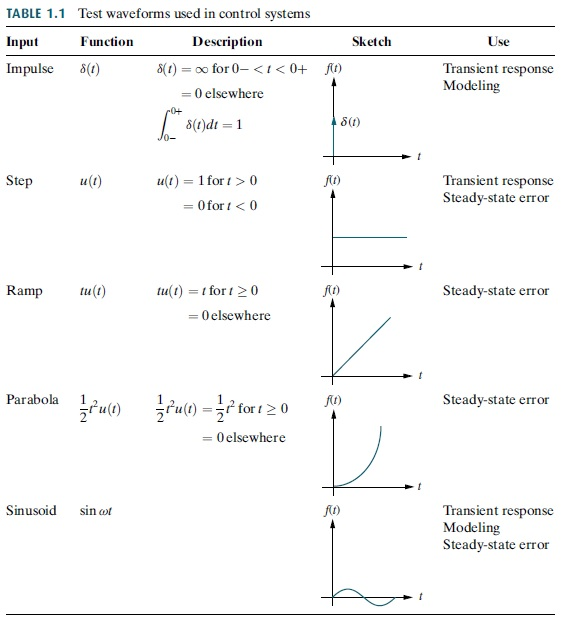
\includegraphics[ width = 0.56\textwidth]{table_1-1_test_waveforms.jpg}
\end{figure}

\end{frame}

% =============================================
\begin{frame}[allowframebreaks]
\frametitle{\S 2.1: Block Diagrams}

\begin{figure}
\centering
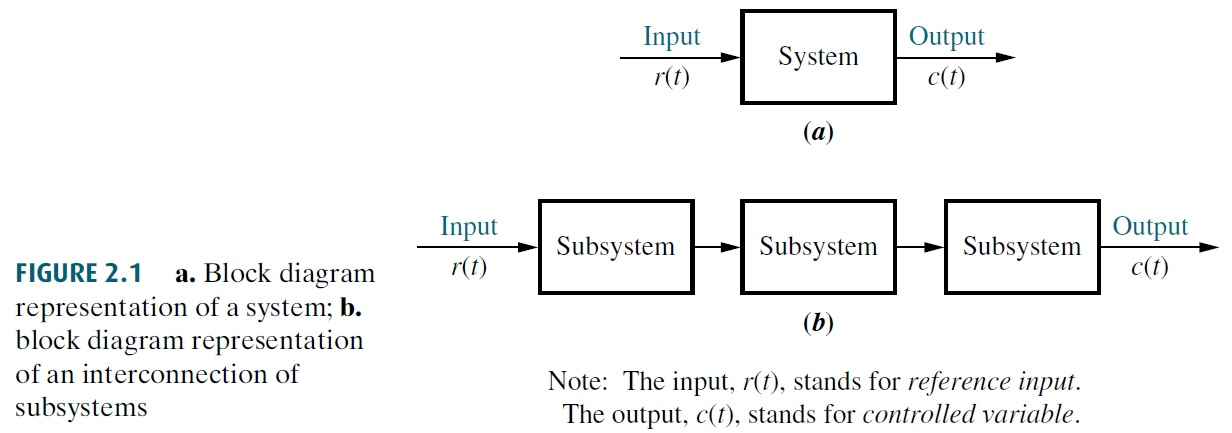
\includegraphics[ width = 0.9\textwidth]{fig_2-1_block_diagrams.jpg}
\end{figure}

\end{frame}

% =============================================
\begin{frame}[allowframebreaks]
\frametitle{\S 2.2: Laplace Transform}

Laplace Transform: 
\begin{itemize}
\item Takes: 
\begin{itemize}
\item A function of time $f(t)$
\item Usually we write the function in lower-case
\end{itemize}
\item Returns: 
\begin{itemize}
\item A function of frequency $F(s)$ such that: 
\[
F(s) \; = \; \mathcal{L}[f(t)] \; = \;
\int_0^{+\infty} f(t) \, e^{-st} \, dt
\]
\item Usually we write the function in upper-case
\end{itemize}
\end{itemize}

\end{frame}

% =============================================
\begin{frame}[allowframebreaks]
\frametitle{\S 2.2: Laplace Transform}

Inverse Laplace Transform: 
\begin{itemize}
\item Takes a function of frequency $F(s)$ and returns a function of time $f(t)$ \linebreak such that: 
\[
f(t) \; = \; \mathcal{L}^{-1}[F(s)] \; = \; 
\frac{1}{ 2 \pi j} \int_{ \sigma - j\infty }^{ \sigma + j\infty } F(s) \, e^{st} \, ds
\]
\halfcut
\begin{itemize}
\item Here, $\sigma$ is any real number greater than the real part of all singularities \linebreak of the function $F(s)$. 
\end{itemize}
\item Clearly, evaluating it from first principles is very painful! 
\item Better idea: Let's make tables of Laplace transforms of various functions \linebreak and then whenever we need to evaluate inverse Laplace transforms \linebreak we simply match $f(t)$ with $F(s)$. 
\end{itemize}

\end{frame}

% =============================================
\begin{frame}[allowframebreaks]
\frametitle{\S 2.2: Laplace Transform Table}

\begin{figure}
\centering
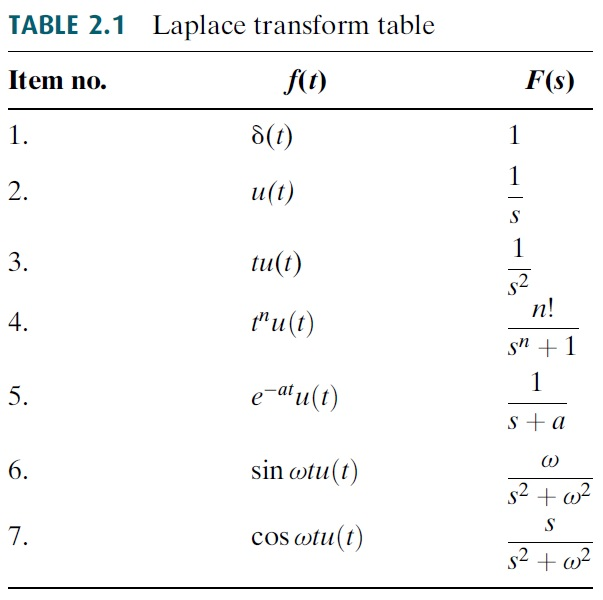
\includegraphics[ width = 0.5\textwidth]{table_2-1_laplace_transform.jpg}
\end{figure}

\end{frame}

% =============================================
\begin{frame}[allowframebreaks]
\frametitle{\S 2.2: Laplace Transform Theorems}

\begin{figure}
\centering
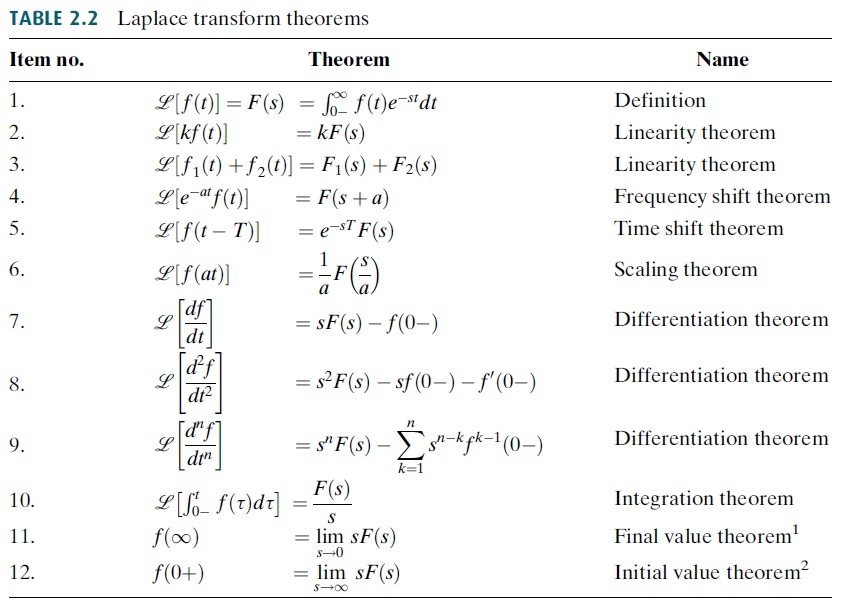
\includegraphics[ width = 0.8\textwidth]{table_2-2_laplace_theorems.jpg}
\end{figure}

\end{frame}

% =============================================
\begin{frame}[allowframebreaks]
\frametitle{\S 2.2: In-class Examples}

\textbf{Problem:} Find the Laplace transform of: 
\[
f(t) = A \, e^{-at} \, u(t)
\]

\textbf{Problem:} Find the Laplace transform of: 
\[
F(s) = \frac{1}{(s+3)^2}
\]

\end{frame}

% =============================================
\begin{frame}[allowframebreaks]
\frametitle{\S 2.2: Partial Fraction Expansion}

\begin{itemize}
\item To find the inverse Laplace transform of a complicated function, we can convert the function to a sum of simpler terms for which we know the Laplace transform of each term. 
\begin{itemize}
\item This might require us to do \href{https://www.mathsisfun.com/algebra/polynomials-division-long.html}{long division}. 
\end{itemize}
\item Consider a function in the frequency domain $F_1(s)$ with numerator $N(s)$ \linebreak and denominator $D(s)$, \iec 
\[
F(s) \; = \; \frac{N(s)}{D(s)}
\]
\item If the order of $N(s)$ is less than the order of $D(s)$, then we are ready to perform a partial-fraction expansion. 
\begin{itemize}
\item \Eg the following function is ready for expansion: 
\[
F(s) \; = \; \frac{2}{s^2+3s+2}
\]
\end{itemize}
\framebreak
\item If the order of $N(s)$ is greater than or equal to the order of $D(s)$, then \linebreak before performing a partial fraction expansion $N(s)$ must be divided by $D(s)$ successively until the result has a remainder whose numerator is of order \linebreak less than its denominator. 
\begin{itemize}
\item \Eg the following function is not ready for expansion: 
\[
F(s) \; = \; \frac{ s^3 + 2s^2 + 6s + 7 }{ s^2 + s + 5 }
\]
So to prepare it for expansion, we write it as follows: 
\[
F(s) \; = \; (s+1) + \frac{2}{ s^2 + s + 5 }
\]
\end{itemize}
\end{itemize}

\end{frame}

% =============================================
\begin{frame}[allowframebreaks]
\frametitle{\S 2.2: Partial Fraction Expansion}

Regarding the Partial Fraction Expansion itself, there are four possible cases \linebreak which depend on the roots of $D(s)$ : 
\begin{enumerate}
\item All roots are real and distinct. 
\begin{itemize}
\item This case is usual in over-damped systems. 
\end{itemize}
\item All roots are real but some are repeated. 
\begin{itemize}
\item This case may occur in critically-damped systems. 
\end{itemize}
\item Some roots are real and others are complex, but all are distinct. 
\begin{itemize}
\item This case is usual in under-damped systems. 
\item Notice that in this case all complex roots appear in conjugate pairs! 
\begin{itemize}
\item \Eg if $s = 1+j$ is a root then $s = 1-j$ must also be a root. 
\end{itemize}
\end{itemize}
\item Some roots are real and others are complex, and some roots are repeated. 
\begin{itemize}
\item This case is extremely rare, both in toy problems and in the real world. 
\end{itemize}
\end{enumerate}

\end{frame}

% =============================================
\begin{frame}[allowframebreaks]
\frametitle{\S 2.2: Partial Fraction Expansion - Case 1}

\begin{itemize}
\item Suppose $F(s)$ is of the form 
\[
F(s) \; = \; 
\frac{N(s)}{ (s+p_1) \, (s+p_2) \, \cdots \, (s+p_n) }
\]
where the roots $p_1, \, p_2, \, \dots, \, p_n$ are all real. 
\item Then, we wish to find $K_1, \, K_2, \, \dots, \, K_n$ such that: 
\[
F(s) \; = \; 
\frac{K_1}{s+p_1} + \frac{K_2}{s+p_2} + \cdots + 
\frac{K_n}{s+p_n}
\]
\item To find $K_1$, we notice the following: 
\[
F(s) \, (s+p_1) \; = \; 
K_1 + \frac{K_2 \, (s+p_1)}{s+p_2} + \cdots + 
\frac{K_n \, (s+p_1)}{s+p_n}
\]
\framebreak
\item Hence, we can use the following ``limit trick'' to compute $K_1$ : 
\[
K_1 \; = \; 
\lim_{ s \rightarrow -p_1 } \; F(s) \, ( s + p_1 )
\]
\item Similarly, we can compute the other constants as follows: 
\begin{align*}
K_2 \; 
& = \; \lim_{ s \rightarrow -p_2 } \; F(s) \, ( s + p_2 ) \\
& \quad \vdots \\
K_n \; 
& = \; \lim_{ s \rightarrow -p_n } \; F(s) \, ( s + p_n )
\end{align*}
\item Finally, to compute the inverse Laplace transform $\mathcal{L}^{-1}$ of $F(s)$ recall that $\mathcal{L}^{-1}$ is linear and that: 
\[
\mathcal{L}^{-1} \left[ \, \frac{K}{s+p} \, \right] \; = \; 
K \, e^{-pt}
\]
\fullcut
\end{itemize}
\fullcut

\end{frame}

% =============================================
\begin{frame}[allowframebreaks]
\frametitle{\S 2.2: Partial Fraction Expansion - Case 1}

\textbf{Problem:} Compute the inverse Laplace transform of: 
\[
F(s) \; = \; \frac{2}{(s+1)(s+2)}
\]

\textbf{Problem:} Use the Laplace transform and its inverse to solve the following differential equation for $y(t)$ assuming all initial conditions are zero. 
\[
\frac{d^2y(t)}{dt^2} + 12 \frac{dy(t)}{dt} + 32y(t) \, = \, 32 u(t)
\]

\end{frame}

% =============================================
\begin{frame}[allowframebreaks]
\frametitle{\S 2.2: Partial Fraction Expansion - Case 2}

\begin{itemize}
\item Suppose $F(s)$ is of the form 
\[
F(s) \; = \; 
\frac{N(s)}{ (s+p_1) \, (s+p_2)^2 }
\]
where the roots $p_1, \, p_2$ are all real. 
\item Then, we wish to find $K_1, \, K_{21}, \, K_{22}$ such that: 
\[
F(s) \; = \; 
\frac{K_1}{s+p_1} + \frac{K_{21}}{s+p_2} 
+ \frac{K_{22}}{(s+p_2)^2}
\]
\item Evidently, we can compute $K_1$ and $K_{22}$ directly using the ``limit trick'': 
\begin{align*}
K_1 \; 
& = \; \lim_{ s \rightarrow -p_1 } \; F(s) \, ( s + p_1 ) \\
K_{22} \; 
& = \; \lim_{ s \rightarrow -p_2 } \; F(s) \, ( s + p_2 )^2
\end{align*}
\framebreak
\item Finally, to find $K_{21}$ we observe that: 
\begin{align*}
& \frac{d}{ds} \left[ \, F(s) \, ( s + p_2 )^2 \, \right] \\[2ex]
& = \; \frac{d}{ds} \left[ \, K_1 \frac{(s+p_2)^2}{s+p_1} + K_{21} \, (s+p_2) + K_{22} \, \right] \\[2ex]
& = \; 
\frac{ 2 \, K_1 \, (s+p_2) }{s+p_1} 
- \frac{ K_1 \, (s+p_2)^2 }{(s+p_1)^2} \; + K_{21} + 0
\end{align*}
\item Therefore, $K_{21}$ can be computed as follows: 
\[
K_{21} \quad = \quad 
\lim_{ s \rightarrow -p_2 } \;
\frac{d}{ds} \left[ \, F(s) \, ( s + p_2 )^2 \, \right]
\]
\end{itemize}

\end{frame}

% =============================================
\begin{frame}[allowframebreaks]
\frametitle{\S 2.2: Partial Fraction Expansion - Case 2}

\begin{itemize}
\item More generally, suppose $F(s)$ is of the form 
\[
F(s) \; = \; 
\frac{N(s)}{ (s+p_1)^{r_1} \, (s+p_2)^{r_2} \, \cdots \, 
(s+p_n)^{r_n} }
\]
where the roots $p_1, \, p_2, \, \dots, \, p_n$ are all real. 
\item Then, we wish to find $K_{11}, \dots, \, K_{1 r_1}, \, K_{21}, \, \dots, \, K_{2 r_2}, \, \dots, \, K_{n1}, \, \dots, \, K_{n r_n}$ \linebreak such that: 
\begin{align*}
F(s) \; 
& = \; \frac{K_{11}}{s+p_1} \; + \; \cdots 
\; + \; \frac{K_{1 r_1}}{(s+p_1)^{r_1}} \\
& \, + \; \frac{K_{21}}{s+p_2} \; + \; \cdots 
\; + \; \frac{K_{2 r_2}}{(s+p_2)^{r_2}} \\[1ex]
& \, + \; \cdots \\[1ex]
& \, + \; \frac{K_{n1}}{s+p_n} \; + \; \cdots 
\; + \; \frac{K_{n r_n}}{(s+p_n)^{r_n}}
\end{align*}
\item If the $i$\tsup{th} root is repeated 2 times we can find $K_{i1}$ and $K_{i2}$ as follows: 
\begin{align*}
K_{i2} \quad 
& = \quad \lim_{ s \rightarrow -p_i } \; 
F(s) \, ( s + p_i )^2 \\
K_{i1} \quad 
& = \quad  \lim_{ s \rightarrow -p_i } \; 
\frac{d}{ds} \left[ \, F(s) \, ( s + p_i )^2 \, \right]
\end{align*}
\item If the $i$\tsup{th} root is repeated 3 times we can find $K_{i1}$, $K_{i2}$ and $K_{i3}$ as follows: 
\begin{align*}
K_{i3} \quad 
& = \quad \lim_{ s \rightarrow -p_i } \; 
F(s) \, ( s + p_i )^3 \\
K_{i2} \quad 
& = \quad  \lim_{ s \rightarrow -p_i } \; 
\frac{d}{ds} \left[ \, F(s) \, ( s + p_i )^3 \, \right] \\
K_{i1} \quad 
& = \quad  \lim_{ s \rightarrow -p_i } \; 
\frac{d^2}{ds^2} \left[ \, F(s) \, ( s + p_i )^3 \, \right]
\end{align*}
\item And so on so forth... 
\framebreak
\item Finally, to compute the inverse Laplace transform $\mathcal{L}^{-1}$ of $F(s)$ recall that $\mathcal{L}^{-1}$ is linear and that: 
\begin{align*}
& \mathcal{L}^{-1} \left[ \, \frac{K}{s+p} \, \right] 
\; = \; K \, e^{-pt} \\[2ex]
& \mathcal{L}^{-1} \left[ \, \frac{K}{(s+p)^2} \, \right] 
\; = \; K \, t \, e^{-pt} \\[2ex]
& \mathcal{L}^{-1} \left[ \, \frac{K}{(s+p)^3} \, \right] 
\; = \; \frac{K}{2} \, t^2 \, e^{-pt} \\[2ex]
& \; \vdots \\[2ex]
& \mathcal{L}^{-1} \left[ \, \frac{K}{(s+p)^m} \, \right] 
\; = \; \frac{ K \, m }{ m! } \, t^{m-1} \, e^{-pt}
\end{align*}
\fullcut
\end{itemize}
\fullcut

\end{frame}

% =============================================
\begin{frame}[allowframebreaks]
\frametitle{\S 2.2: Partial Fraction Expansion - Case 2}

\textbf{Problem:} Compute the inverse Laplace transform of: 
\[
F(s) \; = \; \frac{10}{s(s+2)(s+3)^2}
\]

\end{frame}

% =============================================
\begin{frame}[allowframebreaks]
\frametitle{\S 2.2: Partial Fraction Expansion - Case 3}

\begin{itemize}
\item For any $\alpha, \beta, \gamma \in \Re$ the second-order polinomial $p(x) \, = \, \alpha \, x^2 + \beta \, x + \gamma$ \linebreak has two complex roots if and only if $\beta^2 < 4 \alpha \gamma$. 
\begin{itemize}
\item In this case its roots are: 
\[
x_1 \; = \; 
\frac{-\beta + \sqrt{ \beta^2 - 4 \, \alpha \, \gamma }}{2 \, \alpha} \qquad \qquad
x_2 \; = \; 
\frac{-\beta - \sqrt{ \beta^2 - 4 \, \alpha \, \gamma }}{2 \, \alpha}
\]
\end{itemize}
\item Therefore, the second-order polinomial $p(s) \, = \, s^2 + a \, s + b$ has two \linebreak complex roots if and only if $a^2 < 4b$. 
\begin{itemize}
\item In this case its roots are: 
\[
s_1 \; = \; 
\frac{-a + \sqrt{ a^2 - 4b }}{2} \qquad \qquad
s_2 \; = \; 
\frac{-a - \sqrt{ a^2 - 4b }}{2}
\]
\end{itemize}
\end{itemize}

\end{frame}

% =============================================
\begin{frame}[allowframebreaks]
\frametitle{\S 2.2: Partial Fraction Expansion - Case 3}

\begin{itemize}
\item Suppose $F(s)$ is of the form 
\[
F(s) \; = \; \frac{K_{11} \, s + K_{12}}{s^2 + as + b}
\]
where $a^2 < 4b$. 
\item Then, we don't need carry partial fraction expansion. To see why, \linebreak notice the following: 
\begin{align*}
& \mathcal{L} \left[ \, A \, e^{-\sigma t} \, \cos( \omega t ) \, u(t) \, \right] \; = \; 
\frac{ A \, ( s + \sigma ) }{ (s + \sigma)^2 + \omega^2 } \\[2ex]
& \mathcal{L} \left[ \, B \, e^{-\sigma t} \, \sin( \omega t ) \, u(t) \, \right] \; = \; 
\frac{ B \, \omega }{ (s + \sigma)^2 + \omega^2 }
\end{align*}
\framebreak
\item Consecuently, if $a^2 < 4b$ then 
\[
\mathcal{L}^{-1} \left[
\, \frac{K_{11} \, s + K_{12}}{s^2 + as + b} \, \right] 
\; = \; 
e^{-\sigma t} \, 
( \, A \cos ( \omega t ) + B \sin ( \omega t ) \, ) \, u(t)
\]
where: 
\begin{align*}
& \sigma \; = \; a/2 \\
& \omega \; = \; \sqrt{ b - a^2/4 } \\
& A \; = \; K_{11} \\
& B \; = \; \frac{ K_{12} - A \, \sigma }{\omega}
\end{align*}
\end{itemize}

\end{frame}

% =============================================
\begin{frame}[allowframebreaks]
\frametitle{\S 2.2: Partial Fraction Expansion - Case 3}

\begin{itemize}
\item Now suppose $F(s)$ is of the form 
\[
F(s) \; = \; 
\frac{N(s)}{ (s+p_1) \, ( s^2 + as + b ) }
\]
where $N(s)$ is of degree zero or one, the root $p_1$ is real, and $a^2 < 4b$. 
\item Then, we wish to find $K_1, \, K_{21}, \, K_{22}$ such that: 
\[
F(s) \; = \; 
\frac{K_1}{s+p_1} + 
\frac{K_{21} s + K_{22}}{s^2 + as + b}
\]
\item Evidently, we can still compute $K_1$ directly using the ``limit trick'': 
\[
K_1 \; = \; \lim_{ s \rightarrow -p_1 } \; F(s) \, ( s + p_1 )
\]
\framebreak
\item Once $K_1$ has been found, we can find $K_{21}$ and $K_{22}$ by equating $N(s)$ with \linebreak the numerator of $F(s)$ and then matching coefficients: 
\begin{align*}
N(s) \; 
& = \; K_1 \, ( s^2 + as + b ) 
+ ( K_{21} s + K_{22} ) \, (s+p_1) \\
& = \; 
( K_1 + K_{21} ) \, s^2 + ( K_1 a + K_{21} p_1 + K_{22} ) \, s + ( K_1 b + K_{22} p_1 )
\end{align*}
\item \Eg if $N(s) \, = \, c_2 \, s^2 + c_1 \, s + c_0$ then: 
\begin{align*}
& K_1 + K_{21} \; = \; c_2 \\
& K_1 a + K_{21} p_1 + K_{22} \; = \; c_1 \\
& K_1 b + K_{22} p_1 \; = \; c_0
\end{align*}
\item Finally, the inverse Laplace transform is computed by first recalling that $\mathcal{L}^{-1}$ is linear and then using the formulae presented in the second-to-last slide. 

\end{itemize}

\end{frame}

% =============================================
\begin{frame}[allowframebreaks]
\frametitle{\S 2.2: Partial Fraction Expansion - Case 3}

\textbf{Problem:} Compute the inverse Laplace transform of: 
\[
F(s) \; = \; \frac{3}{ s \, ( s^2 + 2s + 5 ) }
\]

\end{frame}

\end{document}

% =============================================
\begin{frame}[allowframebreaks]
\frametitle{\S 2.4: Electrical Network Transfer Functions}

\textbf{Typical Problem:}

Find the transfer function relating the capacitor voltage, $V_C(s)$, to the input voltage, $V(s)$ in Figure 2.3. 

\begin{figure}
\centering
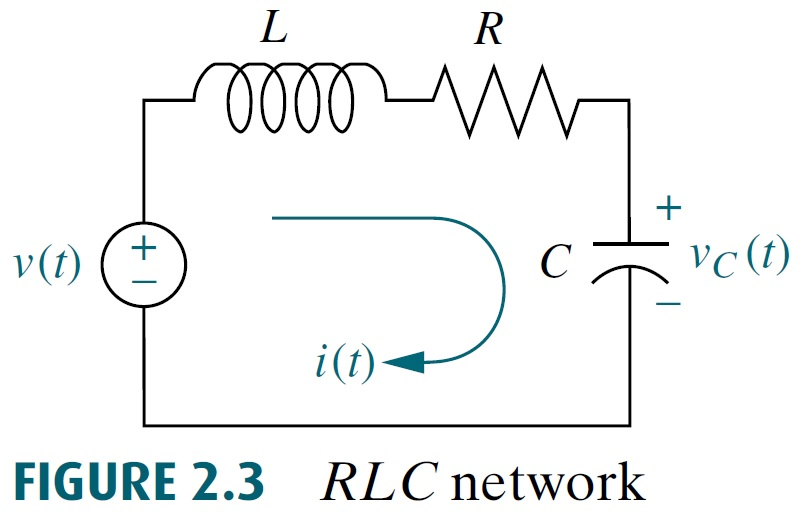
\includegraphics[ width = 0.4\textwidth]{fig_2-3.jpg}
\end{figure}

\end{frame}

% =============================================
\begin{frame}[allowframebreaks]
\frametitle{\S 2.4: Electrical Network Transfer Functions}

How can we write the transfer functions for these problems?
\begin{itemize}
\item Mesh Analysis
\begin{itemize}
\item Use Kirchhoff's Voltage Law (KVL): ``The directed sum of voltages around any closed loop is zero.''
\item We \textbf{write differential equations around loops}, and we write as many \linebreak equations as we need to solve the problem. 
\end{itemize}
\item Nodal Analysis
\begin{itemize}
\item Use Kirchhoff's Current Law (KCL): ``At any node of an electrical circuit \linebreak the sum of currents flowing into that node is equal to the sum of currents flowing out of the node.''
\item We \textbf{write differential equations at nodes}, and we write as many equations \linebreak as we need to solve the problem. 
\end{itemize}
\end{itemize}

\end{frame}

% =============================================
\begin{frame}[allowframebreaks]
\frametitle{\S 2.4: Electrical Network Transfer Functions}

Relations for writing differential equations for electrical circuits: 

\begin{figure}
\centering
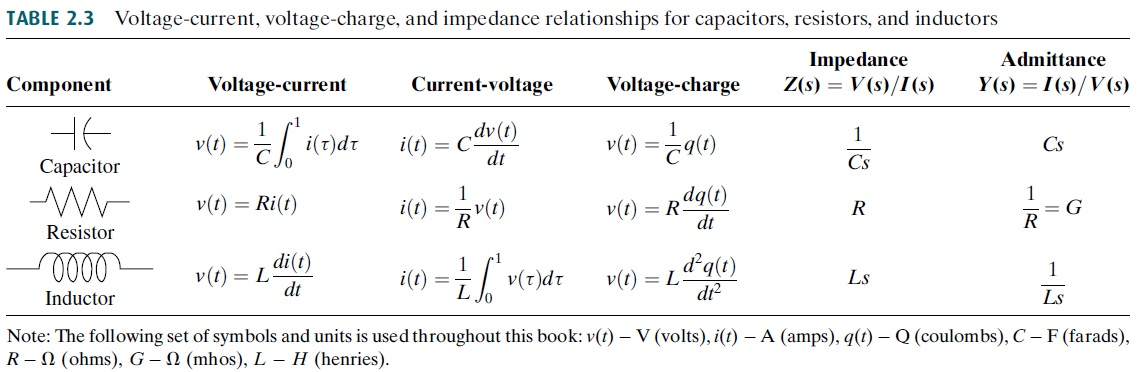
\includegraphics[ width = 0.98\textwidth]{table_2-3.jpg}
\end{figure}

\end{frame}

\end{document}
